\documentclass[tikz,border=10pt]{standalone}
\begin{document}
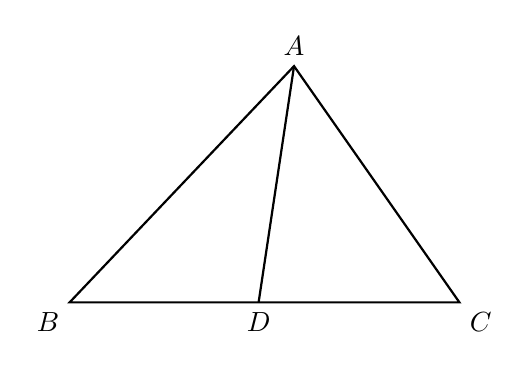
\begin{tikzpicture}[thick, scale=1.5]
    % 定义点坐标
    % B位于原点，C位于(3,0)，A根据一般三角形选取坐标
    \coordinate (B) at (0,0);
    \coordinate (C) at (3.3,0);
    \coordinate (D) at (1.6,0); % 点D在BC上，稍偏向C点
    \coordinate (A) at (1.9,2); % 设置顶点A的位置
    
    % 绘制三角形边线
    \draw (B) -- (C) -- (A) -- cycle;
    
    % 绘制分割线AD
    \draw (A) -- (D);
    
    % 标注顶点
    \node[below left] at (B) {$B$};
    \node[below] at (D) {$D$};
    \node[below right] at (C) {$C$};
    \node[above] at (A) {$A$};
    
\end{tikzpicture}
\end{document}